\documentclass[a4paper,10pt, bibliography=totocnumbered]{scrreprt}

\usepackage[utf8x]{inputenc}
\usepackage[english]{babel}

\usepackage{graphicx}
\usepackage{pdfpages}
%\usepackage{subfig}
%\usepackage{microtype}
\usepackage{tabularx}
%\usepackage{amsmath, textcomp}

% Custom packages
\usepackage[numbers]{natbib}
\usepackage{longtable}
\usepackage{ragged2e}
%\usepackage{tikz}
%\usetikzlibrary{positioning}
%\usepackage{pdflscape}
%\usepackage{rotating}

\usepackage{glossaries} 

\usepackage{hyperref}
\hypersetup{
    colorlinks=true,        % false: boxed links; true: colored links
    linkcolor=black,        % color of internal links
%    citecolor=green,        % color of links to bibliography
    citecolor=black,        % color of links to bibliography
    filecolor=magenta,      % color of file links
    urlcolor=blue           % color of external links
}

% packages Max Edinger
\usepackage{listings}
\usepackage{xcolor}
\usepackage{array}
\usepackage{booktabs}
\newcommand{\tabitem}{~~\llap{\textbullet}~~}
\usepackage{multirow}
\usepackage{pdflscape}
\usepackage[pass]{geometry}


% define colors and configure listing
\colorlet{mygray}{black!30}
\colorlet{mygreen}{green!60!blue}
\colorlet{mymauve}{red!60!blue}
\lstset { %
    language=C++,
    backgroundcolor=\color{gray!10},  
    basicstyle=\ttfamily,
    columns=fullflexible,
    breakatwhitespace=false,      
    breaklines=true,                
    captionpos=t,                    
    commentstyle=\color{mygreen},
    emph={aspect, advice, pointcut, before, JoinPoint}, emphstyle={\color{blue}},
    extendedchars=true,              
    frame=single,                   
    keepspaces=true,             
    keywordstyle=\color{blue},      
    language=c++,                 
    numbers=none,                
    numbersep=5pt,                   
    numberstyle=\tiny\color{blue}, 
    rulecolor=\color{mygray},        
    showspaces=false,               
    showtabs=false,                 
    stepnumber=1,                  
    stringstyle=\color{mymauve},    
    tabsize=3,                      
    title=\lstname,
    numbers=left
}

%% Title Page
\makeatletter
\renewcommand{\maketitle}{\begin{titlepage}
    \vskip 10\p@
    \hbox{
      \vrule depth 0.99\textheight
        \mbox{\hspace{2em}}
      \vtop{
        \vskip 10\p@
        \hspace{4pt}
        \vskip 50\p@
        \begin{flushleft}
          \Large \@author \par
        \end{flushleft}
        \vskip 50\p@
        \begin{flushleft}
          \huge \bfseries \@title \par
        \end{flushleft}
        \begin{flushleft}
          \Large \bfseries \@subtitle \par
        \end{flushleft}
        \vskip 70\p@
        \begin{flushleft}
          \Large \@publishers \par
        \end{flushleft}
        \vskip 50\p@
        \begin{flushleft}
          \Large \@date \par
        \end{flushleft}
        }}
  \end{titlepage}
}
\makeatother

\author{Author 1, Author n}
\title{Title }
\subtitle{Technical Report}
\publishers{\textbf{Advisor University of Heidelberg}\\ Prof. Dr. Barbara Paech, Astrid Rohmann}
\date{mm dd, year}



% Deutsche Absaetze:
\parindent 0pt
\parskip 12pt

\textwidth145mm
\setlength{\oddsidemargin}{0.7cm}
\setlength{\topmargin}{-0.5cm}
\setlength{\textheight}{22.5cm}

\begin{document}
\maketitle

\begin{abstract}
\section*{Abstract}

Testing is an essential and time-consuming part of any software development.
This work is a collaboration that highlights various approaches to how systematic tests can be created to make this process more efficient, clearer, easier or more successful.
After the introduction for this purpose eight different methods are dealt with in own subchapters.
Each of these chapters deals with the investigated approach, describes the problem, discusses the literature search on the topic, and then compares the approaches found in each case via a synthesis matrix.
The approaches are put into practice using the example of a movie manager.
Subsequently, the topic described in this subchapter is summarized and a statement regarding the usage for a systematic test generation is made. 

The first topic dealt with is \enquote{systematic generation of acceptance tests that are executable with FitNesse}.
It is about generating automatic tests with the tool FitNesse.
This approach tries to solve the difficulties of communication among the participants.
For this purpose several artifacts like the fit tables are created and used.
After the investigation, it is concluded that the approaches can work well depending on the project size and experience, but unfortunately it is highly dependent on the latter in particular. 

The next chapter discusses that it should be possible to generate test cases in early phases of development.
\enquote{Transition systems} can help to derive test cases from specifications.
The approaches examined here offer industry standard solutions, but the capability of generating robustness tests for fault detection is still a weakness.

The third subchapter deals with \enquote{Testing with a timing component}.
The difficulty of integrating individual software components into an overall project is described as a problem.
The aspect particularly considered here is the temporal component, since in many real-time systems the exact time between two instruction executions can lead to different results.
After an analysis, the conclusion is drawn that this is still a rarely used approach with many non-automated working steps. 

In the next chapter, approaches for model-based systems are examined.
First and foremost, these include \enquote{classification trees}.
The goal is to derive automatic test cases based on the requirements and the input parameters of a model.
In conclusion, classification trees are described as well arranged and close to the requirements, but can potentially produce many test cases.
Moreover, it is difficult to apply these approaches to systems without a simulated model.

The fifth subchapter focuses on \enquote{model based testing} and examines approaches to make testing with models better and describes the differences between system models and test models.
After the analysis the difficulties in using the tools given in literature are worked out.
Nevertheless, it is possible to reduce test time and errors by using them. 

The initial problem for the next chapter with \enquote{Testing functional and nonfunctional requirements in User Requirements Notation} is the risk for wrong test cases during manual test creation.
User requirements notation should fulfill requirements during test creation and thus prevent incorrect or incomplete tests.
At the end, the problem is discussed that this approach is largely unexplored.
Provided that one makes the effort to take additional steps in test case generation, one still achieves a better quality.

In \enquote{Testing Non-Functional Requirements with Risk Analysis} the focus is on risk analysis, because it is precisely here that error-prone components can be discovered.
Suitable approaches are then sought.
Among the findings here are the importance of automated tests and that tests for non-functional requirements should have more priority. 

The last chapter describes the \enquote{Testing Non-Functional Requirements with Aspects} and puts thereby in the comparison with the previous section the focus on the \enquote{aspects}.
This is intended to describe system-wide functionalities in order to be able to deal with concerns at system level.
Also here the missing availability of tools and suitable research are criticized.
However, the approaches considered seem promising and should be further refined.

Thus, this joint work addresses the merits and difficulties of various test case generation techniques.
Common problems identified are the lack of availability of tools or research, but in suitable use cases most approaches help in improving or automating the test cases.
A final conclusion on this is drawn at the end of this work.

\end{abstract}

\tableofcontents

\chapter{Introduction}\label{sec:introduction}

% Reviewfragen
% - Weckt die Einleitung das Interesse der LeserInnen am Thema?
% - Enthält die Einleitung eine detaillierte Problembeschreibung
%   der Herausforderungen in der Softwareentwicklung, die mit systematischer
%   Testerstellung adressiert werden sollen?
% - Enthält die Einleitung die wesentlichen Aussagen aus den Einleitungen der einzelnen Kapitel?

% Die Einleitung (1 Introduction) des Berichts soll das Interesse der LeserInnen
% am Thema wecken und die gemeinsamen Grundlagen beschreiben. Sie enthält eine
% detaillierte Problembeschreibung der Herausforderungen in der Softwareentwicklung,
% die durch systematische Testerstellung adressiert werden sollen. Zudem enthält sie
% die wesentlichen Aussagen aus den Einleitungen der einzelnen Kapitel 
\section{Systematic Software Testing}\label{sec:introduction_software_testing}

With the rise of smart gadgets and the Internet of Things, more and more parts of our daily life involve technology.
And the software required to run our smartphones, computers and other gadgets  becomes more complex as more data can be processed.
As software becomes more complex, bugs and even small configuration mistakes can have immense consequences as recent data breaches have shown\footnote{\enquote{235 Million Instagram, TikTok And YouTube User Profiles Exposed In Massive Data Leak}, \url{https://www.forbes.com/sites/daveywinder/2020/08/19/massive-data-leak235-million-instagram-tiktok-and-youtube-user-profiles-exposed/}, last visited on 2021-02-10}.
Furthermore, not testing software can have legal consequences.
If basic security measures are not implemented and tested, businesses may violate the \enquote{General Data Protection Regulation}\footnote{see \url{https://eur-lex.europa.eu/legal-content/EN/TXT/?uri=CELEX\%3A02016R0679-20160504&qid=1614251901149}, last visited on 2021-02-25}
(GDPR) and may have to pay fines.
This is not a hypothetical risk.
The \enquote{GDPR Enforcement Tracker}\footnote{see \url{https://www.enforcementtracker.com/}, last visited on 2021-02-10} lists instances where businesses had to pay fines due to \enquote{Insufficient technical and organisational measures to ensure information security}.

Therefore, proper testing of software becomes more important than ever.
But what is software testing? According to the \enquote{Guide to the Software Engineering Body of Knowledge} (short: SWEBOK), \enquote{Software testing consists of the dynamic verification that a program provides expected behaviors on a finite set of test cases, suitably selected from the usually infinite execution domain.}~\cite{SWEBOK}
This means that it may not even be possible to test every input against the expected output, for example if the input is an infinite data stream.
But also for functionality with a finite set of input data, testing every possible combination may not be feasible.
Software testing can take more time than developing the program under test. Hence, software testing can be tedious, difficult and expensive.
So the question arises how software can be tested in an effective and efficient way.

We need to write tests in a systematic way.
This paper contains 9~articles, % TODO: Hat einer aufgehört?
each describing another approach to systematic software testing.

In \autoref{sec:topic_2} % Fitnesse
we focus on acceptance tests with FitNesse.
Communicating requirements between customers and developers can be difficult.
Whereas natural language can be too ambiguous, code can be too technical.
By using FitNesse, human-readable Fit-Tables which include test steps are created that can be understood by customers. By writing fixture classes, these Fit-Tables can be used to automatically run tests.

But having tests may not be enough.
Which requirement is covered by which test?
Can we be sure that the implementation matches the specification?
Traceability becomes necessary and is required to not loose overview over the tests cases and covered requirements.
This is where
\autoref{sec:topic_3} % Transition System
comes into play with transition systems which can be used to automatically create test paths through the application by using formal specifications.

% Notes: Often specification and implementation does not match; traceability issues: which requirement is covered by which test? Solution: Transition system;

After that,
\autoref{sec:topic_4} % Timing Component
looks into testing with a timing component, since for real-time systems, timing is crucial.
In real-time systems, the exact time between two instructions or variances in the individual execution time can lead to different system reactions and therefore different results.

% The aspect particularly considered here is the temporal component, since in many real-time systems the exact time between two instruction executions or variances in the individual execution time can lead to different results.

% Notes: some times issue can only be found if components are linked together; test with same input but different execution time can lead to different reactions in a real-time system.

Following this,
\autoref{sec:topic_5} % Classiciation Tree
looks into decreasing the number of test cases by using classification trees.
Because testing all possible parameter cases becomes unmanageable very fast, these classification trees offer a great way to reduce the complexity of such parameter constructs.
Furthermore, these classification trees can be used to generate test cases.

% Notes: Testing all possible cases becomes unmanageable very fast.Classification Trees offer an approach to offer an approach to reduce the complexity of such parameter con-structions  and  to  keep  them  clearly  arranged.  Test cases can be generated from CTs

\autoref{sec:topic_6} %TODO % Formal specification
\textit{is missing}
% Noch nicht online

In \autoref{sec:topic_7} %  System models
we then look into testing with systems models which are compared against test models.
It is looked into model based testing and how traceability can be used to increase the probability of finding errors and improve test quality.

% KEIN autoref, da sonst kleingeschrieben
Chapter~\ref{sec:topic_8} % NFR/FR Use Requiremetn
explains why writing manual tests for functional and non-functional requirements can be  not only tedious but error prone due to Copy\,\&\,Paste of errors in test logic.
The section describes how test cases can be automatically created by using the user requirements notation that is used for modeling, analyzing, and controlling the correctness and completeness of functional and non-functional requirements.

Another aspect of testing non-functional requirements can be by using risk analysis.
This is where \autoref{sec:topic_9} %  Risk Analysis NFR
steps in and briefly shows how non-functional requirements can be tested and how risk analysis can be used to prioritize test cases.
The section also shows how architectural non-functional requirements such as code conventions can be tested.
\autoref{sec:topic_10} % NFR Aspects
expands on this topic by introducing aspects and aspect oriented programming to test and verify non-functional requirements such as software memory limits and memory leaks.

Finally, \autoref{chap:conclusion} concludes this paper and summarizes each article.

% die Beschreibung der gemeinsamen Grundlagen unter Nutzung des Glossars
% und der Wissensgebiete aus SWEBOK. Das Kapitel gibt einen Überblick über
% die Struktur des Berichts.
\section{Common Fundamentals}\label{sec:introduction_common_fundamentals}
All chapters build upon a common set of fundamental definitions regarding software testing and requirements.
They are listed and mapped to the individual topics in the glossary section of this report.
It is highly recommended to refer to the glossary before reading a chapter or when ambiguities arise while reading a chapter.
However, since it is quite extensive and also contains more topic-specific definitions, the most important terms are defined hereafter.

Like a part of the entries in the glossary section, we use the SWEBOK in its third version as a basis.
Although this guide is already quite old (at least the original version from 2004), hence not fully compliant with current research results, its 15 knowledge areas and basic definitions of a body of knowledge are still useful for classifying the approaches presented in this report and establish a common set of technical terms.

% KEIN autoref, da sonst kleingeschrieben
Let us begin with requirements.
The corresponding SWEBOK knowledge area is \enquote{Software Requirements}.
Relevant sub chapters are \enquote{Software Requirements Fundamentals} and \enquote{Requirements Validation}.
The guide defines requirements as \enquote{a property that must be exhibited by something in order to solve some problem in the real world. [\ldots]
An essential property of all software requirements is that they be verifiable as an individual feature as a functional requirement or at the system level as a non-functional requirement.
It may be difficult or costly to verify certain software requirements.} \cite{SWEBOK}
This definition already points out the difficulty of verifying requirements that necessitates the use of systematic testing techniques, as explained in Section 1.1.
Moreover, it distinguishes between functional requirements, representing a feature the software is to provide, and non-functional requirements, specifying the extend of quality.
Requirements need to be formulated clearly, unambiguously and quantitatively in order to implement and verify them correctly \cite{SWEBOK}.

For software testing, there is no uniform definition.
Therefore, the guide refers to multiple definitions from cited references.
In essence, software testing is to assure that specified requirements are met by the implementation or, from a different perspective, find errors indicating that a requirement has not been met.
This testing process is performed at different levels, as the requirements definition already touched upon.
The SWEBOK guide distinguishes between three test levels: unit testing, verifying isolated functionalities (mostly functional requirements), integration testing, verifying the correct interaction of components and system testing, verifying the behavior of the entire system (mostly non-functional requirements).
Correspondingly, these levels are distinguished by the object of the test (single module, multiple modules, entire system), called the target of the test, and the purpose, called objective of the test \cite{SWEBOK}.

The guide presents a wide array of testing techniques.
For this report, it is important to take notice of the definition of model-based testing: \enquote{A model in this context is an abstract (formal) representation of the software under test or of its software requirements [...].
Model-based testing is used to validate requirements, check their consistency, and generate test cases focused on the behavioral aspects of the software.}\cite{SWEBOK}
Some of the approaches presented in this report are model based, at least partially.
However, it is not always clear what the actual model is and some authors use the term incorrectly.

\section{Outline}
\label{sec:intruduction1.3}

Following this introduction in \autoref{sec:introduction}, nine individual reports each present two different but related approaches for systematic testing in Chapters 2\,-\,10.
The reports introduce their superordinate topic in Sections X.1, outline the results and execution of a literature search based on a given article in Sections X.2 and describe the given and selected approach in Sections X.3.1 and X.4.1 as well as illustrating them using a common set of given requirements in Sections X.3.2 and X.4.2.
Finally, the approaches are compared using a common set of synthesis questions in Sections X.5 and evaluated in Sections X.6.
Chapter 11 concludes the report.
The glossary and bibliography can be found in Chapters 12 and 13.\\

In the following, the given requirements (\autoref{fig:mm}) and synthesis questions, used for each individual report, are depicted.

\newpage
\textbf{Synthesis questions:}

\begin{enumerate}
	\item Description of the approach (What does the approach do?)
	\begin{enumerate}
		\item Which artifacts and relations between artifacts are used in this approach? Which artifacts are created in the course of the approach? How are the artifacts characterized?
		\item What is required and/or input for the application of the approach?
		\item What steps does the approach consist of? Which information is used in which step and how? What are the results of the individual steps?
	\end{enumerate}
	\item[] 
	\item Benefits of the approach (Whom does the approach help and how?)
	\begin{enumerate}
		\item Which usage scenarios are supported by the approach?
		\item Which stakeholders are supported by the usage scenarios?
		\item Which knowledge areas from SWEBOK can be assigned to the usage scenarios?
	\end{enumerate}
	\item Tool support for the approach (What tool support is available?)
	\begin{enumerate}
		\item What tool support is provided for the approach?
		\item Which steps of the approach are automated by a tool? Which steps are supported by a tool, but still have to be executed manually? Which steps are not supported by a tool?
	\end{enumerate}
	\item Quality of the approach (How well does the approach work?)
	\begin{enumerate}
		\item How was the approach evaluated?
		\item What are the (main) results of the evaluation?
	\end{enumerate}
\end{enumerate}


\newpage
\newgeometry{margin=1cm}
\begin{landscape}

\begin{figure}
	\centering
	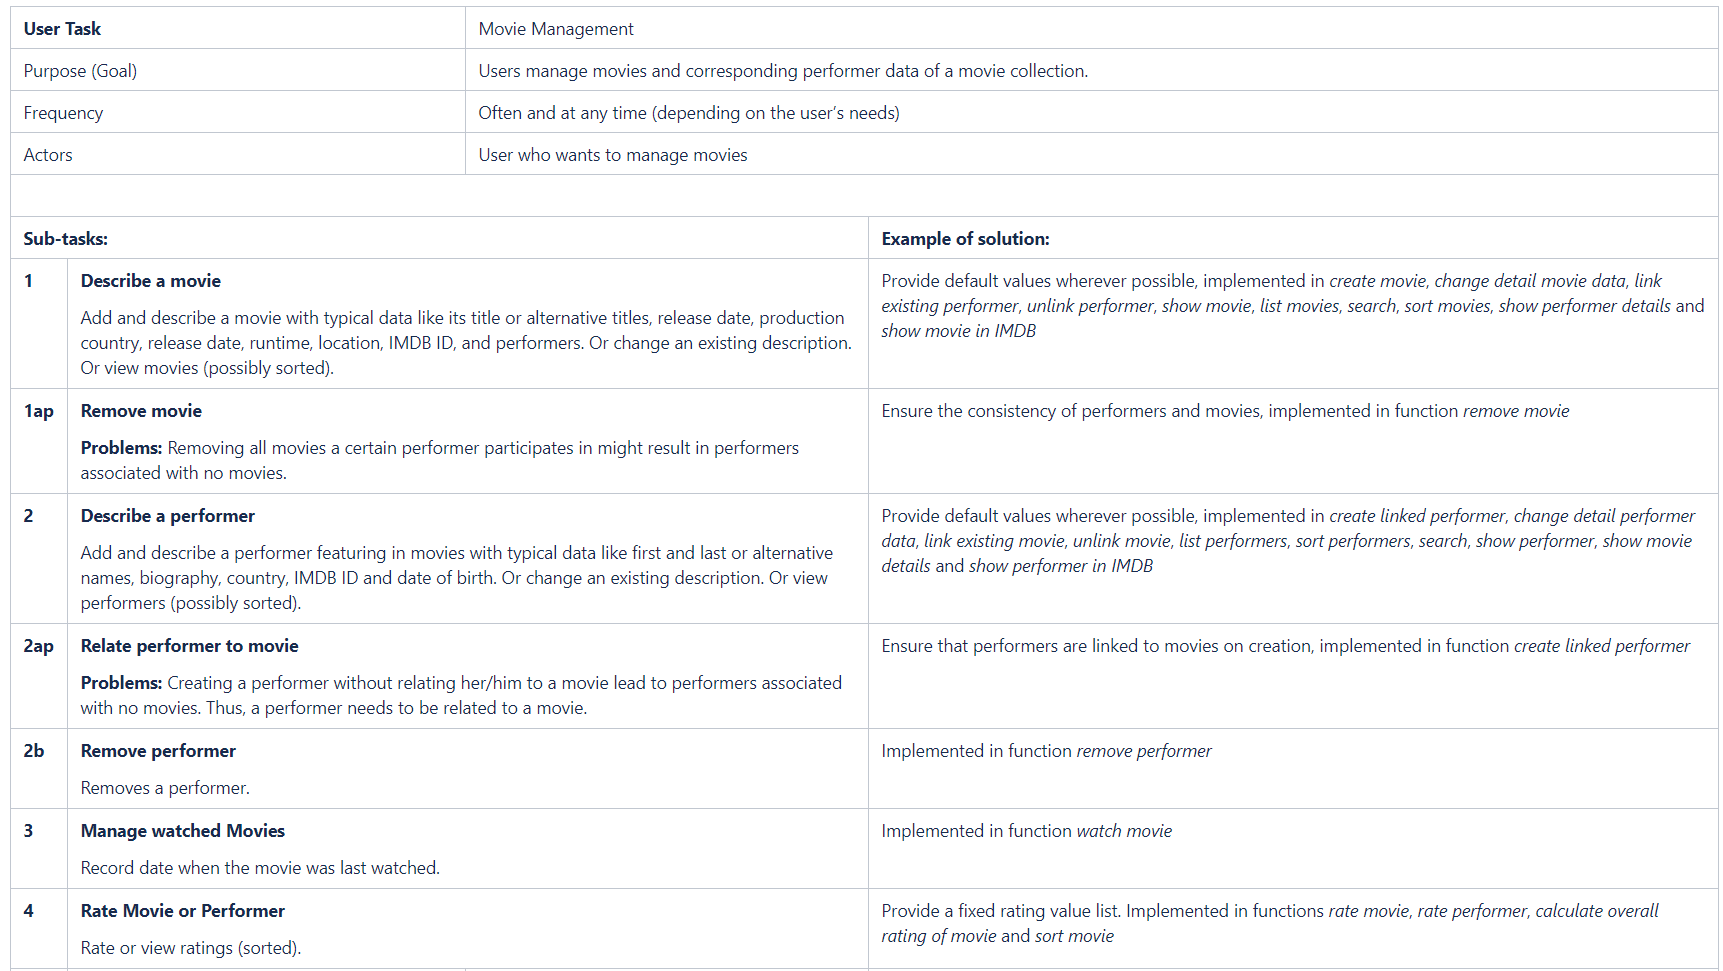
\includegraphics[scale=0.57]{../images/MovieManager.png} 
	\caption{Requirements in User-Task notation for the MovieManager software, an application for managing movie collections.}
	\label{fig:mm}
\end{figure}

\end{landscape}
\restoregeometry



\chapter{Richtiges Zitieren}

1.	Die Seminararbeit ist eine eigenständige wissenschaftliche Arbeit und wird auch nach den Regeln einer wissenschaftlichen Arbeit erstellt (vgl.~\cite{RichtigesZitierenTUDresden}), insbesondere heißt das, dass die Regeln für:
\begin{enumerate}
\item Richtiges Zitieren 
\begin{itemize}
\item Zitierpflicht
\item Zitierregeln
\item Typen von Zitaten
\item Zitierformen
\end{itemize}
\item Literaturangaben 
\item eine gut strukturierte Arbeit 
\end{enumerate}
beachtet und eingehalten werden.




\chapter{Chapter}

Duis porta orci. Integer eu arcu at enim tempus facilisis. Pellentesque dignissim orci sed est. Etiam elementum laoreet mi. Donec nunc sapien, dictum in, tristique sed, aliquam vitae, massa. Morbi magna magna, vestibulum tempor, lobortis non, convallis nec, nibh. In sed nibh. Suspendisse adipiscing dictum pede. Suspendisse non augue. Lorem ipsum dolor sit amet, consectetuer adipiscing elit. Pellentesque lacinia, velit sed commodo convallis, diam dolor consequat ligula, a scelerisque quam neque et purus. Praesent vel augue. Sed lectus leo, dignissim eget, vulputate eu, auctor ut, nulla. Vivamus a quam. Nulla tellus. Pellentesque tempor pulvinar nunc.


\chapter{Testing Non-Functional Requirements with Aspects}

\section{Introduction}

Software testing ensures that specified requirements, functional and non-functional, are met by the implementation. Non-functional requirements are especially hard to test because they do not describe what the software does, but how and to what extend of quality it does it. Hence the also customary term quality requirements. They pose numerous challenges for software testing and software quality due to their system-wide effects and often crosscutting nature. They do not only concern one part of the software and its source code, but multiple or even the entire system. For instance, the memory requirement: “The system only uses two gigabytes of main memory at most at all times.” has a restrictive influence on other requirements and system functionality like performance requirements. This impedes the observance of the widely propagated principle of separation of concerns, introduced by Parnas \cite{Parnas} and Dijkstra \cite{Dijkstra}, throughout development and testing.\\
\\
By virtue of the afore-mentioned problems, there are only few tools and systematic approaches for testing non-functional requirements. Frequently, they are evaluated subjectively, resulting in a loss of traceability between test code, source code and requirements. Aspect orientation is a technique that can be harnessed for testing non-functional requirements. It is a programming paradigm, aiming to modularise such requirements (in the context of AOP, they are called system-level concerns in contrast to core-level concerns), similar to the modularisation of functional requirements using objects. An aspect modularises a system-level concern and thereby represents a system-wide functionality, accessible to multiple classes and other parts of the software. Let us consider a common application for AOP: Listing \ref{logging} shows a simple logging aspect in C++. It consists of three main components:
\begin{itemize}
\item Joinpoint: The point in the program code, the aspect is executed. It can be before, after or around something (here: before).
\item Advice: Associates the joinpoint with an activity (here: a printf statement). 
\item Pointcut: Selects a suitable joinpoint out of the set of all joinpoints and associates it with a method or function (here: \%::\%()).
\end{itemize}

\lstset {language=C++}
\begin{lstlisting}[caption={\textbf{Logging Aspect in C++.}}, label=logging]
aspect LoggingAspect{
	public:
		pointcut logMethods() = call("% %::%()");
		advice logMethods() : before(){
			printf("> Enter: %s\n", JoinPoint::signature());
		}
};
\end{lstlisting}

\newpage
In this example, the printf logging statement is executed each time before the \%::\%() method is called. Based on these principles, many possibilities for systematic and automated testing are conceivable.\\
\\
In the following, the execution and results of a literature search based on a given article are presented in Section \ref{lit}. Subsequently, the given article , which assesses the use of aspects for testing non-functional requirements as well as the suitability of certain non-functional requirements for aspect-oriented testing is described and applied to an example in Section \ref{given}. Likewise, for a selected article found using the literature search in Section \ref{found}.  It expands upon the basic ideas of the first article and partially automates the creation of test aspects. Thereafter, the results of a literature comparison are presented in Section \ref{compare}. Finally, in Section \ref{feierabend} both approaches as well as the general concept of testing using aspects are evaluated. 

\section{ Literature Search} \label{lit}

To find relevant literature, a literature research based on the following search question was conducted: \textbf{\textit{Which approaches for systematic creation of tests (for non-functional requirements) using aspects exists?}} Both forward and backward snowballing proceeding from the given article as well as a term-based search were carried out. The used terms were test, aspects, AOP and aspect-oriented. Restrictions to reduce the number of hits are described in Table \ref{restrict}. First, the upper term from Table \ref{restrict} with everything in the publication title was used, then the lower term from Table \ref{restrict} with test in the title, aspects in the abstract and AOP and aspect-oriented in all meta data. Source platforms for the search were IEEE and ACM. IEEE because the given article as well as articles referencing it can be found here. ACM because there are many available and peer-reviewed articles differing from IEEE. Content-based relevance criteria were derived directly from the search question:

\begin{itemize}
\item The article must cover the creation of tests using aspects because this is the main topic of the given article. Furthermore, the criterion is used to exclude articles covering testing of aspect-oriented software with conventional methods.
\item The article must describe systematic approaches for the creation of tests, since this is the superordinate topic of the seminar. 
\item The article must describe test methods for non-functional requirements, as this is the subtopic of the given article.
\end{itemize}

In addition to these content-based criteria, there were some rather soft criteria:
\begin{itemize}
\item The article must be from different authors.
\item The article must be written in English or German language.
\end{itemize}

\begin{table}[h]
\caption{\textbf{Search Terms, Restrictions and Sources.}}
\begin{tabular}{|p{6.5cm}|p{4.5cm}|p{2cm}|}
\hline
\textbf{Term} & \textbf{Restrictions} & \textbf{Sources}\\
\hline
\multirow{2}{8cm}{\textbf{test} AND (\textbf{aspects} OR \textbf{AOP} OR \textbf{aspect-oriented})} & \tabitem all in title  &  \tabitem IEEE\\
& \quad & \tabitem ACM \\
\hline
\multirow{2}{8cm}{\textbf{test} AND \textbf{aspects} AND \textbf{AOP} AND \textbf{aspect-oriented}} & \tabitem test in title  &  \tabitem IEEE\\
& \tabitem aspects in abstract & \tabitem ACM \\
\hline
\end{tabular}
\label{restrict}
\end{table}

Table \ref{doc} shows the execution and results of the literature search. For further selection, the relevant articles were divided into three categories:

\begin{itemize}
\item overviews of testing using aspects,
\item examples for testing using aspects,
\item improvement or monitoring of conventional (unit) test using aspects. 
\end{itemize}

The given article can be classified between overview and example. Via the literature search, I wanted to find an article providing automation and tool support, seen as the given article has shortcomings in that regard. Moreover, all relevance criteria must be fulfilled and it would be beneficial if the article covers at least two out of three classification categories.\\
\\
Many articles violate the first criteria, because they cover the testing of aspect-oriented software without using aspects. Some articles were not chosen because they just cover one classification category, therefore not really adding new information and approaches.\\
\\
The article that stood out was Duclos et al.: “ACRE: An Automated Aspect Creator for Testing C++ Applications” \cite{Duclos} because it covers all categories and satisfies all criteria. It includes an extensive general section followed by the description of an approach for automated creation of test aspects on an example to improve or replace conventional tests. Since the article was found using forward snowballing, it directly references the given article and proposes solutions for problems the latter raises. This article was selected.

\newpage
\newgeometry{margin=1cm}
\begin{landscape}

\begin{table}
\caption{\textbf{Literature Research Documentation.}}
\begin{longtable}{|p{1.3cm}|p{1.8cm}|>{\raggedright}p{2.3cm}|>{\raggedright}p{6cm}|p{1.5cm}|p{1.5cm}|p{1.2cm}|p{2cm}|}

\hline
\textbf{Source} & \textbf{Date} & \textbf{Restrictions} & \textbf{Term} & \textbf{Results} & \textbf{Relevant} & \textbf{Used} & \textbf{Comments}\\
\hline
IEEE$^*$ & 11.11.2020 & none & forward snowballing & 10 & 5 & $\nabla$ & -\\
\hline
IEEE$^*$ & 11.11.2020 & none & backward snowballing & 22 & 5 & none & -\\
\hline
IEEE$^*$ & 11.11.2020 & none & "All Metadata":test AND ("All Metadata": aspects OR "All Metadata":AOP OR "All Metadata":aspect-oriented) & 220,605 & ? & none & too general, not considered\\
\hline
ACM$^\dagger$ & 11.11.2020 & none & [All: test] AND [[All: aspects] OR [All: aop] OR [All: aspect-oriented]] & 172,120 & ? & none & too general, not considered\\
\hline
IEEE$^*$ & 11.11.2020 & title &"Document Title":test AND ("Document Title": aspects OR "Document Title":AOP OR "Document Title":aspect-oriented) & 158 & 11 & none & first 50 considered\\
\hline
ACM$^\dagger$ & 12.11.2020 & title &[Publication Title: test] AND [[Publication Title: aspects] OR [Publication Title: aop] OR [Publication Title: aspect-oriented]] & 311 & 4 & none & first 50 considered\\
\hline
IEEE$^*$ & 12.11.2020 & test: title, aspects: abstract &((("Document Title":test) AND "Abstract":aspects) AND "All Metadata":AOP) AND "All Metadata":aspect-oriented & 33 & 16 & none & -\\
\hline
ACM$^\dagger$ & 12.11.2020 & test: title, aspects: abstract &[Publication Title: test] AND [Abstract: aspects] AND [All: aop] AND [All: aspect-oriented] & 31 & 6 & none & -\\
\hline
\end{longtable}
\textit{\qquad \qquad \qquad \qquad \qquad *: https://ieeexplore.ieee.org/Xplore/home.jsp \quad $\dagger$: https://dl.acm.org/ \quad $\nabla$: \cite{Duclos}}
\label{doc}
\end{table}

\end{landscape}
\restoregeometry

\newpage
\section{Metsä et al.: “Testing Non-Functional Requirements with Aspects: An Industrial Case Study” } \label{given}

\subsection{Description}
The research article “Testing Non-Functional Requirements with Aspects: An Industrial Case Study” by Jani Metsä of Nokia in association with Mika Katara and Tommi Mikkonen \cite{Metsa} of Tampere University of Technology was published in 2007 as part of the Seventh International Conference on Quality Software. According to the authors, the main goal of software testing is to ensure that requirements are met by the implementation. There are already several systematic approaches for testing functional requirements, but only few for testing non-functional requirements. To tackle this problem, they turned to aspect-oriented programming as a potential testing technique. In their paper, they try to answer the following research questions:

\begin{enumerate}
\item To what extent can aspect-oriented techniques be harnessed to test non-functional requirements?
\item Which non-functional requirements lend themselves for testing with aspects?
\end{enumerate}

The authors conducted a case study, analysing 150 requirements of an existing industrial embedded system (a quality verification software for mobile phones running Symbian OS). They were able to identify 16 crosscutting non-functional requirements for which seven test aspects were formulated and implemented. In detail, in the first step, a set of provided system requirements or characteristics are analysed and corresponding non-functional requirements (which might be crosscutting) derived. One non-functional requirement is derived from one or more system requirements, a system requirement can comprise multiple non-functional requirements. In a second step, the non-functional requirements are categorised (performance, robustness, …), and corresponding testing objectives are derived. One testing objective is derived from one or more non-functional requirements. Finally, the test aspects can be formulated based on the testing objectives and non-functional requirements categories. One test aspect can comprise multiple testing objectives.\\  
\\
The approach proved to be easy and test coverage could be increased significantly. The use of aspects enables non-invasive testing throughout the software lifecycle. Furthermore, separation of (test) concerns can be achieved by modularizing crosscutting non-functional requirements. As a result, maintainability, reusability as well as tracing between requirements and test code can be improved.  Based on the experiences gained, the authors concluded that especially system-wide and crosscutting non-functional requirements, such as security, performance, reliability and robustness, are suitable for aspect-oriented testing.
To sum up, the article presents a systematic approach – a systematology - to derive testing objectives and test cases with related test aspects from non-functional requirements. It does not provide automation for any step, hence the main problems the authors identify: the lack of tool support and the need for testing personnel to be firm with aspect-oriented programming.

\newpage
\subsection{Application}

 The non-functional requirements (REQ) are derived from the user task or the corresponding system characteristics (Table \ref{req}). They have system-wide effects (hence affect multiple system-functions) and are of crosscutting nature. For example, REQ5 and REQ6 set performance constraints on REQ7 and REQ8 as well as REQ3; REQ3 and REQ4 set reliability and robustness constraints on each other; REQ9 sets security constraints on REQ1 and REQ2.\\
\\
 Subsequently, the non-functional requirements are categorised and corresponding test objectives can be derived (Table \ref{obj}).\\
\\
Finally, a test aspect for one or multiple requirement categories is formulated (Table \ref{aspects}). These test aspects would then need to be implemented manually using an AOP-Framework (AspectC++ \cite{C++}, AspectJ \cite{J}, …). For instance, the Memory Aspect could work like this: every time the constructor or destructor of an entity class (Movie, Performer, …) is called, a counter will be incremented or decremented by the size of the class.

\begin{table}[h]
\caption{\textbf{Initial System Requirements of the Movie Manager App.}}
\begin{tabular}{|p{7cm}|p{7cm}|}
\hline
\textbf{System Characteristic} & \textbf{Derived Requirement}\\
\hline
\multirow{2}{6.5cm}{Data is managed consistently by the system.} & REQ1: Default values are provided (wherever possible).\\
 & REQ2: Entities are linked consistently (a performer must always be linked to at least one movie).\\ 
\hline  
\multirow{2}{6.5cm}{The system is fault tolerant and able to report faulty behaviour.} & REQ3: The system can recover from hang situations.\\
 & REQ4: The system can identify correct and incorrect system behaviour.\\
\hline 
\multirow{2}{6.5cm}{The system runs on a mobile phone with limited amount of resources and thus has a strict memory footprint.} & REQ5: The system must occupy at maximum W bytes of ROM\\
 & REQ6: The system must occupy at maximum X bytes of RAM.\\
\hline 
\multirow{2}{6.5cm}{The system is fast and responsive.} & REQ7: The system can respond to requests after Y time units after power-up.\\
 & REQ8: All user requests are handled in Z time units.\\
\hline  
The system might hold sensitive data and is therefore secure. & REQ9: The system follows the Android App security best practices (e.g. a password is required for sensitive data changes).\\
\hline
\end{tabular}
\label{req}
\end{table}

\begin{table}
\caption{\textbf{Testing Objectives for Non-Functional Requirements.}}
\begin{tabular}{|p{2cm}|p{8cm}|p{4cm}|}
\hline
\textbf{REQ} & \textbf{Testing Objective} & \textbf{Requirement Category}\\
\hline
REQ1 & TO1: Supervise data consistency and integrity. & Security (Integrity).\\
REQ2 & \quad & \quad \\
\hline
REQ9 & TO2: Check password protection. & Security\\
\hline 
REQ3 & TO3: Generate hang situation. & Robustness\\
\hline 
REQ3 & TO4: Analyse system reliability. & Reliability\\
REQ4 & \quad & \quad \\
\hline 
REQ5 &TO5: Supervise memory consumption. & Performance (Memory)\\
REQ6 & \quad & \quad \\
\hline
REQ7 & TO6: Measure time consumed from power-on to the system being in a responsive state. & Performance\\
\hline 
REQ7 \quad REQ8 &TO7: Measure time consumed on serving requests and executing system-functions. & Performance\\
\quad & \quad & \quad \\
\hline
\end{tabular}
\label{obj}
\end{table}

\begin{table}
\caption{\textbf{Formulated Test Aspects.}}
\begin{tabular}{|p{4cm}|p{8cm}|p{2cm}|}
\hline
\textbf{Test Aspect} & \textbf{Description} & \textbf{Test Objective(s)}\\
\hline
Integrity Aspect & Checks if all specified default values are provided and performers are linked to at least one movie. & TO1\\
\hline
Security Aspect & Tries to execute all data changing system-functions without providing the password. It should ‘t be possible to commit the changes. & TO1, TO2\\
\hline
Robustness Aspect & Generates a request jam to test if the SUT can recover from the hang situation. & TO3\\
\hline
Reliability Aspect & Collects information on SUT states and failures. & TO4\\
\hline
Memory Aspect & Supervise memory consumption by tracking all memory allocations and deallocations. & TO5\\
\hline
Performance Aspect & Measure function execution times. & TO6, TO7\\
\hline
\end{tabular}
\label{aspects}
\end{table}

\newpage
\section{Duclos et al.: “ACRE: An Automated Aspect Creator for Testing C++ Applications” } \label{found}

\subsection{Description}

Etienne Duclos, Sébastien Le Digabel, Yann-Gaël Guéhéneuc and Bram Adams \cite{Duclos} of École Polytechnique de Montréal published their article “ACRE: An Automated Aspect Creator for Testing C++ Applications” in 2013 as part of the 17th European Conference on Software Maintenance and Reengineering. They state that software should be faultless and in accordance with requirements yet testing costs need to be acceptable. Systematic and developer-friendly tools for testing functional and non-functional requirements are required to achieve this goal. However, such tools are sparce, especially for non-functional requirements. The authors review related approaches for testing with aspects, including the approach by Metsä et al., and conclude that high-level tool support and automation are required to solve the problems raised in these publications. To achieve this, they try to answer the following tripartite research question:\\
\\
Can automatically generated test aspects be used to \dots
\begin{enumerate}
\item \dots detect memory leaks?
\item \dots test invariants?  
\item \dots detect interference bugs?
\end{enumerate}

The authors present ACRE (automated aspect creator), a tool that automatically generates test aspect code using a domain specific language. Provided a set of test cases or objectives or a bug report, the DSL statement describing the test aspect can be derived. The type of the bug or the category of the underlying NFR of the test case determines the type of the test aspect that must be chosen in this step. Afterwards, the test aspect is generated automatically based on the DSL description. ACRE takes the entire source code as an input and looks for DSL statements. They are parsed to generate the corresponding test aspects.\\
\\
Using ACRE, the authors were able to detect one error of each type (1. – 3.) in the mathematical optimisation software NOMAD. Thanks to the DSL description of the test aspect, testing personnel does not need to have extensive knowledge about aspect-oriented programming, just about the DSL syntax. Although the creation of test cases from requirements or bug reports is not automated, the DSL and the types of available test aspects provide support in that regard. However, this means that the approach is currently limited to specific use cases (memory leaks, invariants, interference bugs in C++ applications). Nevertheless, it would be easy to extend the available functionalities and transfer the approach to other programming languages with support for aspect-oriented programming. \\
\\
To sum up, the article presents a tool for the automatic generation of test aspects with given test cases formulated in a domain specific language.

\newpage
\subsection{Application}
The non-functional requirements with corresponding test objectives or a bug report must be given, as the approach does not present a way to derive them. Let us consider the same requirements (REQ1-9) and test objectives (TO1-7) as in Table \ref{req} and Table \ref{obj}. Furthermore, a user of the Movie Manager App has filed the following bug report:

\begin{table}[h]
\caption{\textbf{Bug Report.}}
\begin{tabular}{|p{14cm}|}
\hline
\textbf{Summary:} Memory Leak when removing all movies of a performer.\\
\hline
\textbf{Description:} Deleting all Movies linked to a performer leads to the removal of the performer from the performers list, but no memory* is not actually freed.\\
\hline
\textbf{Steps to reproduce:} \begin{enumerate} \item Consider a performer with one linked movie. \item Delete the linked Movie. \end{enumerate}\\
\hline
\textbf{Actual results:} The performer and movie are removed from the respective lists, but no memory is freed.\\
\hline
\textbf{Expected results:} The performer and movie are removed from the respective lists and both objects are no longer in memory.\\ 
\hline
\end{tabular}
\textit{(*For the purpose of this example, let us consider all data is kept in main memory.)}
\label{bug}
\end{table}


Based on the given test objectives or the bug report, the test aspects must be formulated manually using a domain-specific language. However, the DSL provides certain types of Aspects (Counter, Logging, Timing, Checking) and guidelines that help formulate the test cases. Table \ref{aspect-test} shows the aspect types corresponding to the given test objectives and test aspects of approach 1. The DSL formulation to test for memory leaks in the  Performer class  could look like this:

\lstset {language=C++}
\begin{lstlisting}[caption={\textbf{DSL Statement For Counter Aspect}}, label=dsl]
// // name: MemoryAspect              
// // type: Counter                           
// // className: Performer    
// // namespace: MovieManager       
\end{lstlisting}

The parameters \textit{'name'} and \textit{'type'} are required and determine the name and type of the test aspect. 'className' and 'namespace' are optional and specify, which class are concerned by the aspect. By default, the file in which the DSL statement was found is searched for namespaces and the name of the file is considered to be the name of the class.  It must be placed somewhere within the source code, for example above or below the tested function or class or in a separate file. Afterwards, ACRE takes the entire source code as an input, looks for DSL statements (always starting with // //) and generates the corresponding test aspects automatically. For the example above, ACRE generates the memory aspect for the Performer class as shown in Listing \ref{mem}. In essence, the counter aspect initialises a static counter variable that is incremented each time the Performer constructor is called and decremented each time the destructor is called. After the execution of the main method, the final count as well as a warning in case of a memory leak (counter $>$ 0) are printed. In this manner, a class causing a memory leak can be detected. The timing and logging aspects are quite similar to the counter aspect. The checking aspect is more complex and allows the declaration of variables as well as the use of for-loops, while-loops and if-clauses. Note that the timing aspect in its current form is used for interference bug testing, hence it measures access times to variables. However, a timing aspect for measuring function call times could easily be implemented by starting a timer before each function call and stopping it after each function call in the advice of the aspect.

\begin{table}[h]
\caption{\textbf{Aspect Types for Given Test Objectives.}}
\begin{tabular}{|>{\raggedright}p{2cm}|p{8cm}|p{1cm}|p{2cm}|}
\hline
\textbf{Test \quad Aspect} & \textbf{Description} & \textbf{Test Objective(s)} & \textbf{Aspect Type}\\
\hline
Integrity Aspect & Checks if all specified default values are provided and performers are linked to at least one movie. & TO1 & Checking \\
\hline
Security Aspect & Tries to execute all data changing system-functions without providing the password. It should ‘t be possible to commit the changes. & TO1, TO2 & Checking\\
\hline
Robustness Aspect & Generates a request jam to test if the SUT can recover from the hang situation. & TO3 & Checking, Logging\\
\hline
Reliability Aspect & Collects information on SUT states and failures. & TO4 & Logging\\
\hline
Memory Aspect & Supervise memory consumption by tracking all memory allocations and deallocations. & TO5 & Counting\\
\hline
Performance Aspect & Measure function execution times. & TO6, TO7 & Timing (not in current form)\\
\hline
\end{tabular}
\label{aspect-test}
\end{table}

\lstset {language=C++}
\begin{lstlisting}[caption={\textbf{Generated Counter Aspect Code.}}, label=mem]
aspect MemoryAspect{
	public static int _Eval_Performer = 0;

	pointcut Eval_Performer() = "MovieManager::Performer";
	advice Eval_Performer() : slice struct{
		class Eval_Performer{
			public:
				// constructor -> increment
				Eval_Performer(){
					MemoryAspect::_EvalPerformer++;
				}
				// destructor -> decrement
				~Eval_Performer(){
					MemoryAspect::_EvalPerformer--;
				} 
		} 
	};

	// print counter (and warning)
	advice execution (main(...)) : after () {
		printf("Final count of Eval_Performer: \%d\n",  _Eval_Performer)
		if(_Eval_Performer > 0)
			printf("Memory Leak! \n")
	}
};
\end{lstlisting}

\newpage
\section{Comparison} \label{compare}

The approaches have been compared using a set of synthesis questions, as shown in Table \ref{syn}.\\
\\
Both approaches offer the same benefits: using test aspects, it is possible to test system-wide crosscutting non-functional requirements in a non-invasive way (without modifying or instrumentalising the source code). As a result, modularity, maintainability reusability as well as traceability of requirements to corresponding tests can be improved. Multiple stakeholders can benefit from both approaches, in particular testing and maintenance personnel. Correspondingly, both approaches use and produce similar artifacts: test objectives are derived from requirements and ultimately implemented using aspects.\\
\\
However, there are differences concerning the specific individual steps, the level of automation as well as the relating quality of the approaches. Approach 1 describes a systematology to derive aspect test cases from requirements. These have to be implemented manually. In contrast, approach 2 assumes the test objectives to be provided and generates corresponding test aspects automatically. Subsequently, the most significant difference is the tool support: approach 1 does not provide any tool support, but rather describes a systematology. Approach 2 fully automates the final step of approach 1 – from test objectives to test code – and assists with the set-up of the concrete test cases through the structure of the domain specific language.\\ 
\\
This is reflected in the evaluation of the respective approach as well. Both draw the conclusion that aspects are well suited for testing non-functional requirements. Approach 1 criticises the lack of tool support, approach 2 counteracts this exact problem. In Summary, the two approaches are quite similar. However, approach 1 is less extensive concerning the automation of the technique and should be regarded as a rather fundamental research. Approach 2 expands on the ideas of approach 1 and enhances their quality by partially automating the process. 

\newpage
\newgeometry{margin=1cm}
\begin{landscape}

\begin{table}
\caption{\textbf{Synthesis Matrix.}}
\begin{longtable}{|p{2cm}|>{\raggedright}p{4cm}|>{}p{8cm}|>{}p{8cm}|}
\hline
Question 
& Name 
& Approach 1: \textbf{Testing Non-Functional Requirements with Aspects} 
& Approach 2: \textbf{ACRE}\\ \hline
%\hline %%%%%%%%%%%%%%%%%%%%%%%%%%%%%%%%%%%%%%%%%%%%%%%%%%%%%%%%
\multirow{3}{*}{3 \rotatebox[origin=r]{90}{\textbf{Description}}} 
& a) artefacts and relationship between artefacts 
& system requirements in natural language (provided), NFRs (derived), testing objectives (derived), test aspects (derived)
& test objectives or bug report (provided), DSL-statements within the source code (derived), test aspects (generated)\\ 
\cline{2-4}
& b) preconditions/ input 
&  system requirements 
& test objectives or bug report\\ 
\cline{2-4}
& c) steps, results, informations 
&  \underline{Step 1}: Provided a set of system requirements, NFRs (which might be crosscutting) are derived. One NFR is derived from one or more system requirements, a system requirement can comprise multiple NFRs. \underline{Step 2}: The NFRs are categorised and corresponding testing objectives are derived. One testing objective is derived from one ore more NFRs. \underline{Step 3}: Test aspects can be formulated based on the testing objectives and NFR categories. One test aspect can comprise multiple testing objectives.
 & \underline{Step 1}: Provided a set of testing objectives or a bug report, the DSL statement describing the test aspect can be derived. The type of the bug or the category of the underlying NFR of the testing objective determines the type of the test aspect that must be chosen in this step. \underline{Step 2}: The test aspect is generated automatically based on the DSL description.\\
\hline %%%%%%%%%%%%%%%%%%%%%%%%%%%%%%%%%%%%%%%%%%%%%%%%%%%%%%%%
\multirow{3}{*}{4 \rotatebox[origin=r]{90}{\textbf{Benefits}}} 
& a) supported usage scenarios 
& Easy and non-invasive testing throughout the software lifecycle: during initial development for debugging or validating NFRs, during system testing and for maintaining tasks. Separation of concerns by modularizing crosscutting NFRs. Tracing of NFRs and corresponding tests 
& Easy and non-invasive testing throughout the software lifecycle: during initial development for debugging or validating NFRs, during system testing and for maintaining tasks. Separation of concerns by modularizing crosscutting NFRs. Tracing of NFRs and corresponding tests\\ 
\cline{2-4}
& b) supported stakeholders 
& Developers, testing and maintenance personnel
& Developers, testing and maintenance personnel\\ 
\cline{2-4}
& c) corresponding SWEBOK-Knowledge Areas
 & Software Requirements (NFRs, Requirements Tracing), Software Testing (System Test), Software Maintenance 
& Software Requirements (NFRs, Requirements Tracing), Software Testing (System Test), Software Maintenance\\ 
\hline %%%%%%%%%%%%%%%%%%%%%%%%%%%%%%%%%%%%%%%%%%%%%%%%%%%%%%%%
\multirow{2}{*}{5 \rotatebox[origin=r]{90}{\textbf{Tools}}} 
& a) tool support 
& none (except the aspects themselves)
&ACRE (Automated Aspect Creator), DSL\\ 
\cline{2-4}
& b) level of automation 
&  none 
& Test cases and testing objectives must be derived manually from the requirements. The DSL facilitates the test case design. The test aspect code is generated automatically from the DSL statements.\\ 
\cline{2-4}
\hline %%%%%%%%%%%%%%%%%%%%%%%%%%%%%%%%%%%%%%%%%%%%%%%%%%%%%%%%
\multirow{2}{*}{6 \rotatebox[origin=r]{90}{\textbf{Quality}}} 
& a) evaluation
& Case study with requirements of an existing industrial embedded system. Comparison of test coverage with and without test aspects.
& An empirical study aiming to find errors in the mathematical optimisation software NOMAD was conducted. The approach was contrasted with other common techniques and tools.\\ 
\cline{2-4}
& b) evaluation results 
& Test aspects proved to be an easy and non-invasive technique for testing NFRs. Seperation of (test) concerns by modularising NFRs.  BUT: lack of tool support, complicated build process. 
& Automatically generated test aspects proved to be suitable for finding memory leaks, interference bugs and testing invariants. The approach is easy to use because developers do not need to know aspect-oriented programming itself, only the DSL syntax and semantics. BUT: derivation of test cases from requirements and DSL statement input still manual\\ 
\cline{2-4}
\hline %%%%%%%%%%%%%%%%%%%%%%%%%%%%%%%%%%%%%%%%%%%%%%%%%%%%%%%%
\end{longtable}
\label{syn}
\end{table}

\end{landscape}
\restoregeometry

\newpage
\section{Conclusion} \label{feierabend}

In summary, this report presents two articles describing possible approaches to harness aspect-oriented techniques for testing non-functional requirements. A literature search based on the first article was carried out to obtain an overview of the current state of research and find relevant literature for this report. The selected article builds upon the ideas of the given article and presents a tool for (partially) automating the creation of test aspects. The two approaches have been compared and illustrated using a literature synthesis with a set of synthesis questions and a synthesis matrix as well as an application to an example.\\
\\ 
The results of both research articles and the synthesis and example, conducted for the report, indicate that aspects are suitable for testing non-functional requirements in a systematic manner due to multiple reasons: Firstly, the basic functionality of aspects carries an inherent systematology and lends itself for testing. An aspect comprises a set of statements that can be executed every time before, after or around a function call, which can easily be utilised to check pre- and postconditions or to measure resource consumption and runtimes. In addition to that, they are non-invasive, meaning the tested source code does not need to be modified and the test aspect can easily be separated from the main code, reused or removed. Furthermore, test aspects are especially suitable for testing non-functional requirements because they modularise the system level concerns, non-functional requirements pose, thus maintaining separation of concerns. System-wide functionality, that is spread out through the entire system and its source code can be tested using one aspect. This also improves traceability between the non-functional requirements and the corresponding tests.\\
\\ 
Metsä et al. point out that the lacking tool support and the need for developers to have a firm understanding of aspect-oriented programming pose possible challenges. Duclos et al. solve these problems (partially) by introducing ACRE, a tool that parses DSL statements to generate test aspects automatically.  However, the tool only supports four aspect types and is limited to C++ applications. The lack of subsequent research articles (after 2013) indicates that systematic testing using aspects is not in focus of current research anymore. Nevertheless, existing approaches and tools, as presented in this report, should be further refined to make use of the aforementioned advantages of aspect-oriented testing, especially for non-functional requirements. Because aspect-oriented programming lost popularity in recent years, applying aspect-oriented testing techniques in practice is difficult because only few developers and testers are able to implement them. However, using a domain specific language as an intermediate layer of abstraction, as described by Duclos et al, tackles this problem and enables relevant stakeholders to use test aspects as small, re-usable and none-invasive test modules throughout the software lifecycle at the system test level. 






\chapter{Conclusion}
Fusce vitae quam eu lacus pulvinar vulputate. Suspendisse potenti. Aliquam imperdiet ornare nibh. Cras molestie tortor non erat. Donec dapibus diam sed mauris laoreet volutpat. Sed at ante id nibh consectetuer convallis. Suspendisse diam tortor, lobortis eget, porttitor sed, molestie sed, nisl. Integer enim nisl, lacinia in, pretium eu, viverra a, odio. Quisque at quam eget risus placerat porttitor. Suspendisse convallis, elit vitae mattis pharetra, orci nisl ultrices sapien, ac interdum metus lorem iaculis diam. Nunc id nunc sit amet nisl tincidunt congue. Curabitur et sapien.

%% Bibliography
\bibliographystyle{plainnat}
%\bibliography{literature.bib}%Bibliography file name

\begin{thebibliography}{9}

\bibitem{C++} AspectC++ Development Team: About the Project.
\url{https://www.aspectc.org/} last accessed 2020/12/28

\bibitem{KunChen2005} Chen, K, Zhang, W., Zhao, H.: An approach to constructing feature models based on requirements clustering.
In: 13th IEEE International Conference on Requirements Engineering (RE05). pp. 31-40. (2005)

\bibitem{Dijkstra} Dijkstra, E.: A Discipline of Programming.
In: Prentice-Hall Series in Automatic Computation Englewood Cliffs, New Jersey. (1976)

\bibitem{Duclos} Duclos, E., Le Digabel, S., Guéhéneuc, Y.,  Adams, B.: "ACRE: An Automated Aspect Creator for Testing C++ Applications“.
In:  CSMR 2013 Genova.  pp. 121-130. (2013). \url{10.1109/CSMR.2013.22}

\bibitem{J} Eclipse Foundation: AspectJ.
\url{https://www.eclipse.org/aspectj/}  last accessed 2020/12/28

\bibitem{RichtigesZitierenTUDresden} Institut für Geographie   
Lehrstuhl für Allgemeine Wirtschafts- und Sozialgeographie: An Hinweise zum wissenschaftlichen Arbeiten.
\url{http://www.geogr.uni-jena.de/fileadmin/Geoinformatik/Lehre/backup_05_2007/pdf-dokumente/Skript_WissArbeiten.pdf}

\bibitem{Metsa} Metsä, J., Katara, M., Mikkonen, T.: "Testing Non-Functional Requirements with Aspects: An Industrial Case Study“.
In:  QSIC 2007 Portland. pp. 5-14. (2007). \url{10.1109/QSIC.2007.4385475}

\bibitem{Parnas} Parnas, D.: On the criteria to be used in decomposing systems into modules.
In: Communications of the ACM. (1972)


\end{thebibliography}

\listoffigures

\listoftables

\end{document}          
